\documentclass[conference]{IEEEtran}
\IEEEoverridecommandlockouts
\usepackage{cite}
\usepackage{amsmath}
\usepackage{newtxtext}
\usepackage{newtxmath}
\usepackage{graphicx}
\usepackage{booktabs}
\usepackage{multirow}
\usepackage[hidelinks]{hyperref}
\usepackage{balance}

\begin{document}

\title{\textbf{Cross-Domain Generalization and Lightweight Domain Adaptation for SMS Spam Detection}}

\author{
\IEEEauthorblockN{Dr. Kayarvizhy N}
\IEEEauthorblockA{\textit{Professor} \\ \textit{Department of Computer Science and} \\ \textit{Engineering} \\
\textit{B.M.S. College of Engineering}\\
Bengaluru, India \\
kayarvizhyn.cse@bmsce.ac.in}
\and
\IEEEauthorblockN{Priyam Thakur}
\IEEEauthorblockA{\textit{Department of Computer Science and} \\ \textit{Engineering} \\
\textit{B.M.S. College of Engineering}\\
Bengaluru, India \\
priyamthakur.cs23@bmsce.ac.in}
\and
\IEEEauthorblockN{Bhavya Goyal}
\IEEEauthorblockA{\textit{Department of Computer Science and} \\ \textit{Engineering} \\
\textit{B.M.S. College of Engineering}\\
Bengaluru, India \\
bhavyagoyal.cs23@bmsce.ac.in}
\and
\IEEEauthorblockN{Samir Chaudhary}
\IEEEauthorblockA{\textit{Department of Computer Science and} \\ \textit{Engineering} \\
\textit{B.M.S. College of Engineering}\\
Bengaluru, India \\
samirchaudhary.cs23@bmsce.ac.in}
\and
\IEEEauthorblockN{Sana Subodh}
\IEEEauthorblockA{\textit{Department of Computer Science and} \\ \textit{Engineering} \\
\textit{B.M.S. College of Engineering}\\
Bengaluru, India \\
sanasubodh.cs23@bmsce.ac.in}
}

\maketitle


\begin{abstract}
SMS spam classifiers are usually trained and tested on messages from the same collection, where conventional models report accuracies above 95\%. This paper asks whether such models transfer to an independently collected dataset from a different country, and whether a small labelled sample from the new domain closes the gap. We train Multinomial Naive Bayes and Logistic Regression on word-level and character-level TF-IDF features from the UCI SMS Spam Collection (5,158 unique UK messages) and evaluate them, without retraining, on an Indian SMS dataset (2,050 unique messages). Trained on UCI only, Logistic Regression drops from a spam F1-score of 0.911 on held-out UCI messages to 0.678 on Indian messages, recalling only 53.3\% of Indian spam; Naive Bayes drops from 0.906 to 0.551. Adding 10\% of a labelled Indian adaptation pool (143 messages) to the UCI training data raises the mean target F1 over three seeds from 0.681 to 0.964 for Logistic Regression and from 0.582 to 0.950 for Naive Bayes, without lowering source-domain F1. The improvement occurred in all three seeds and was significant by McNemar's test in each. Because Indian promotional SMS are templated, we also repeat adaptation with near-duplicate groups kept on one side of the split; the gain persists (0.652 to 0.952 for Logistic Regression). Neither feature representation was better for both classifiers.
\end{abstract}

\begin{IEEEkeywords}
SMS spam detection, domain shift, cross-domain generalization, domain adaptation, TF-IDF, Naive Bayes, logistic regression
\end{IEEEkeywords}

\section{Introduction}
Unwanted SMS remain a daily problem, and machine-learning filters for them have a long history. Most published results, however, train and test on random splits of a single collection, most often the UCI SMS Spam Collection~\cite{almeida2011}. On such splits, conventional classifiers and deep models report accuracies between 96\% and 99\%~\cite{almeida2013,roy2020}. These numbers describe performance on messages that resemble the training data. They do not say what happens when a filter built in one place meets messages from another, where vocabulary, brands, currencies, link styles and message length all differ.

This difference between the training distribution and the deployment distribution is called domain shift. Learning theory shows that the error on a new (target) domain depends on the error on the source domain and on how different the two domains are~\cite{bendavid2010}. A common practical remedy, when a few labelled target examples are available, is supervised domain adaptation: adding them to the training data~\cite{daume2007,pan2010}.

We study this question for SMS spam with deliberately simple, conventional tools, so that the effect of the data is not hidden by model complexity. We ask five research questions:
\begin{itemize}
\item \textbf{RQ1}: Does a model trained on one SMS dataset generalize to an independently sourced SMS dataset?
\item \textbf{RQ2}: Which model performs better under cross-domain evaluation?
\item \textbf{RQ3}: Does character-level TF-IDF improve target-domain performance compared with word-level TF-IDF?
\item \textbf{RQ4}: Can a small labelled subset of target-domain messages improve performance?
\item \textbf{RQ5}: Which message characteristics are associated with cross-domain errors?
\end{itemize}

Our contributions are a controlled source-only versus adapted comparison on the same untouched target test set, repeated over three seeds with paired significance tests; an audit of the target dataset; a check that the adaptation gain is not caused by near-duplicate messages shared between the adaptation pool and the test set; and a released notebook and application that reproduce every number reported here.

\section{Related Work}
\textit{SMS spam corpora and classifiers.} Almeida et al.\ released the SMS Spam Collection, 5,574 English messages of which 747 are spam~\cite{almeida2011}, and later compared many classifiers on it, preferring a linear SVM~\cite{almeida2013}. Roy et al.\ report up to 99.44\% accuracy with CNN and LSTM models on the same corpus~\cite{roy2020}. These studies share one dataset and evaluate within it.

\textit{Domain shift and adaptation.} Ben-David et al.\ bound target-domain error by source error plus a measure of divergence between domains~\cite{bendavid2010}. Pan and Yang survey transfer learning, including the setting where a small amount of labelled target data is available~\cite{pan2010}. Daum\'e~III shows that simple ways of combining source and target data are strong baselines for supervised domain adaptation in NLP~\cite{daume2007}. Our adaptation method is the simplest of these: pooling source data with a labelled target sample.

\textit{Evaluation pitfalls.} Near-duplicate text across training and test sets inflates measured performance~\cite{lee2022}, and train--test duplication is one of the most common forms of leakage in applied machine learning~\cite{kapoor2023}. We therefore test whether near-duplicates explain our adaptation gains.

\section{Datasets and Audit}
\textit{Dataset A (source).} The UCI SMS Spam Collection~\cite{almeida2011} (CC~BY~4.0): 5,574 UK messages, 4,827 ham and 747 spam.

\textit{Dataset B (target).} The India Spam SMS Classification dataset, published on GitHub under the MIT licence in 2024~\cite{indiasms}: 2,267 messages with fields \texttt{Msg} and \texttt{Label}, 1,522 ham and 745 spam. Messages were contributed through an online form; the repository does not document a labelling procedure.

\textit{Audit.} Following the project guide's checklist, we checked counts, missing values, duplicates, label conflicts, encoding and provenance (Table~\ref{tab:data}). Dataset B had one empty message and 204 exact duplicates; 176 rows stored emoji and punctuation as broken byte sequences (for example \texttt{ðÂ...}), which we repaired with the ftfy library rather than deleting the rows, and 40 rows had Devanagari text irrecoverably replaced by question marks. No message appeared with two different labels. A spot check of ten messages per class found plausible labels: Indian spam is dominated by operator, bank and retail promotions with links, while ham is mostly short personal or group-chat messages. One message (\textit{``ok''}) occurred in both datasets and was removed from Dataset B.

\begin{table}[t]
\centering
\caption{Datasets before and after cleaning}
\label{tab:data}
\begin{tabular}{lrrrrr}
\toprule
Dataset & Raw & Clean & Ham & Spam & Spam \% \\
\midrule
A: UCI (UK) & 5,574 & 5,158 & 4,517 & 641 & 12.4 \\
B: India & 2,267 & 2,050 & 1,314 & 736 & 35.9 \\
\bottomrule
\end{tabular}
\vspace{2pt}

\footnotesize Cleaning removed 416 duplicates from A, and from B one empty row, 215 duplicates and one message shared with A.
\end{table}

\section{Methodology}
\subsection{Preprocessing}
Labels were mapped to spam $=1$ and ham $=0$. Both datasets received the same light cleaning: broken encodings repaired, text lowercased, leading and trailing spaces stripped, repeated whitespace collapsed and exact duplicates removed. URLs, numbers and punctuation were kept, because they carry spam signals.

\subsection{Features}
A message $d$ is represented by TF-IDF weights~\cite{salton1988}
\begin{equation}
w_{t,d} = \mathrm{tf}_{t,d}\cdot\left(\ln\frac{1+N}{1+\mathrm{df}(t)}+1\right),
\end{equation}
followed by $\ell_2$ normalisation, where $N$ is the number of training messages and $\mathrm{df}(t)$ the number containing term $t$. We compare word unigrams and bigrams (at most 20,000 features) with character 3--5-grams within word boundaries (\texttt{char\_wb}). Every vectorizer is fitted on training data only.

\subsection{Classifiers}
Multinomial Naive Bayes estimates $P(t\mid c)$ with additive smoothing $\alpha$ and predicts the class with the larger posterior. Logistic Regression models $P(y=1\mid x)=\sigma(\mathbf{w}^\top x+b)$ with $\ell_2$ regularisation of strength $1/C$, \texttt{max\_iter} $=1000$ and balanced class weights, justified by the 12.4\% spam share of Dataset A. A linear SVM is included as an optional comparison in the cross-domain test. The hyperparameter of each model and feature set ($\alpha$ or $C$) was chosen by 5-fold stratified cross-validation on Dataset A's training split only, maximising spam F1, and then fixed for every experiment: $\alpha=0.03$ for Naive Bayes, $C=100$ (word) and $C=10$ (character) for Logistic Regression, and $C=1$ for the SVM. All models use scikit-learn 1.7.2~\cite{pedregosa2011}.

\subsection{Experimental Protocol}
Dataset A is split 80/20 into training and test sets, and Dataset B 70/30 into a target adaptation pool (1,435 messages) and a final target test set (615 messages), both stratified. \emph{Source-only} models are trained on A's training split (4,126 messages). \emph{Adapted} models are trained on A's training split plus a stratified sample of 10\%, 20\% or 40\% of the adaptation pool (143, 287 or 574 messages); the vectorizer and classifier are refitted on this combined set. All settings within a seed are scored on the same final target test set, which is never used for training, fitting features or choosing hyperparameters. The whole procedure is repeated with seeds 42, 123 and 2026, and we report mean~$\pm$~standard deviation. A 100\% row is shown only as a reference.

\subsection{Metrics and Statistics}
With spam as the positive class we report accuracy, precision, recall and F1. To compare a source-only and an adapted model on the same test messages, we use the exact McNemar test~\cite{mcnemar1947,dietterich1998}, which counts only the messages that one model classifies correctly and the other does not.

\section{Results}
\subsection{RQ1 and RQ2: Cross-Domain Generalization}
Table~\ref{tab:cross} applies the source-only models of seed 42 to all 2,050 messages of Dataset B. Every model loses between 0.23 and 0.36 F1. Precision on Indian messages stays high (0.88--0.96), but recall falls to 0.40--0.55: the models rarely raise false alarms, but they miss about half of the Indian spam. Logistic Regression with word features transfers best (F1 0.678). Model choice matters less than the domain: the best and worst source-domain F1 differ by 0.04, while every model falls far more on the target domain.

\begin{table}[t]
\centering
\caption{Trained on Dataset A only (seed 42): spam F1 on A's test split and on all of Dataset B}
\label{tab:cross}
\begin{tabular}{llcccc}
\toprule
Model & Feat. & F1$_A$ & F1$_B$ & Prec.$_B$ & Rec.$_B$ \\
\midrule
Naive Bayes & word & 0.906 & 0.551 & 0.883 & 0.401 \\
Logistic Reg. & word & 0.911 & \textbf{0.678} & 0.931 & 0.533 \\
Linear SVM & word & 0.914 & 0.615 & 0.949 & 0.455 \\
Naive Bayes & char & 0.948 & 0.684 & 0.908 & 0.549 \\
Logistic Reg. & char & 0.940 & 0.638 & 0.942 & 0.482 \\
Linear SVM & char & 0.943 & 0.578 & 0.956 & 0.414 \\
\bottomrule
\end{tabular}
\end{table}

The choice of smoothing for Naive Bayes is decisive under domain shift. With the library default $\alpha=1$, Naive Bayes reached F1 0.726 on Dataset A but only 0.014 on Dataset B, labelling almost every Indian message as ham. Choosing $\alpha$ on source data alone raised these to 0.906 and 0.551.

\subsection{RQ4: Lightweight Domain Adaptation}
Table~\ref{tab:adapt} and Fig.~\ref{fig:curve} show the effect of adding labelled Indian messages. Most of the gain comes from the first 10\% of the pool: 143 messages raise mean target F1 from 0.681 to 0.964 for Logistic Regression and from 0.582 to 0.950 for Naive Bayes. Going to 40\% adds a further 0.01--0.03. Source-domain F1 does not fall: it stays near 0.93 for both models. The gain was positive in all three seeds for every model, feature set and fraction, and McNemar's test gave $p<0.05$ in every one of the 36 comparisons. At seed 42, for example, 98 test messages were correct only for the adapted Logistic Regression (40\%) and four only for the source-only model. Fig.~\ref{fig:cm} shows that adaptation mainly converts missed spam into detected spam (Logistic Regression: false negatives 96 $\to$ 3) while false positives stay similar (10 $\to$ 9).

\begin{table}[t]
\centering
\caption{Spam F1 on the final target test set, word TF-IDF, mean $\pm$ SD over three seeds}
\label{tab:adapt}
\begin{tabular}{lcc}
\toprule
Target data added & Naive Bayes & Logistic Regression \\
\midrule
0\% (source-only) & 0.582 $\pm$ 0.018 & 0.681 $\pm$ 0.025 \\
10\% (143 msgs) & 0.950 $\pm$ 0.006 & 0.964 $\pm$ 0.004 \\
20\% (287 msgs) & 0.967 $\pm$ 0.007 & 0.968 $\pm$ 0.005 \\
40\% (574 msgs) & \textbf{0.978} $\pm$ 0.009 & \textbf{0.975} $\pm$ 0.005 \\
\midrule
100\% (reference) & 0.987 $\pm$ 0.007 & 0.987 $\pm$ 0.003 \\
\bottomrule
\end{tabular}
\end{table}

\begin{figure}[t]
\centering
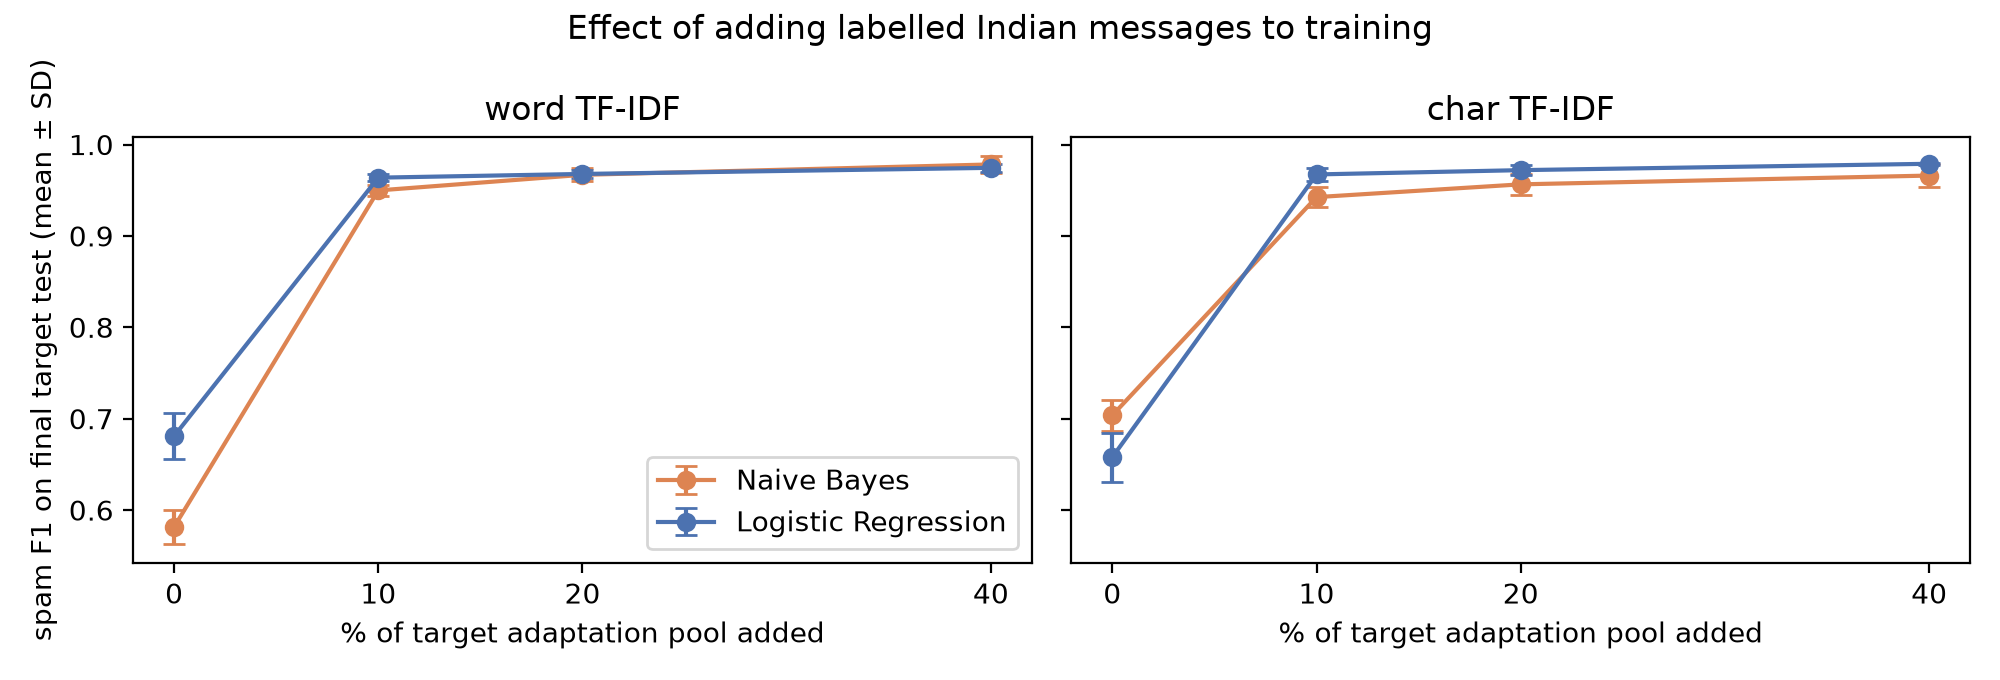
\includegraphics[width=\columnwidth]{figures/fig4_adaptation_curve.png}
\caption{Spam F1 on the final target test set as labelled Indian messages are added (mean $\pm$ SD over three seeds).}
\label{fig:curve}
\end{figure}

\begin{figure}[t]
\centering
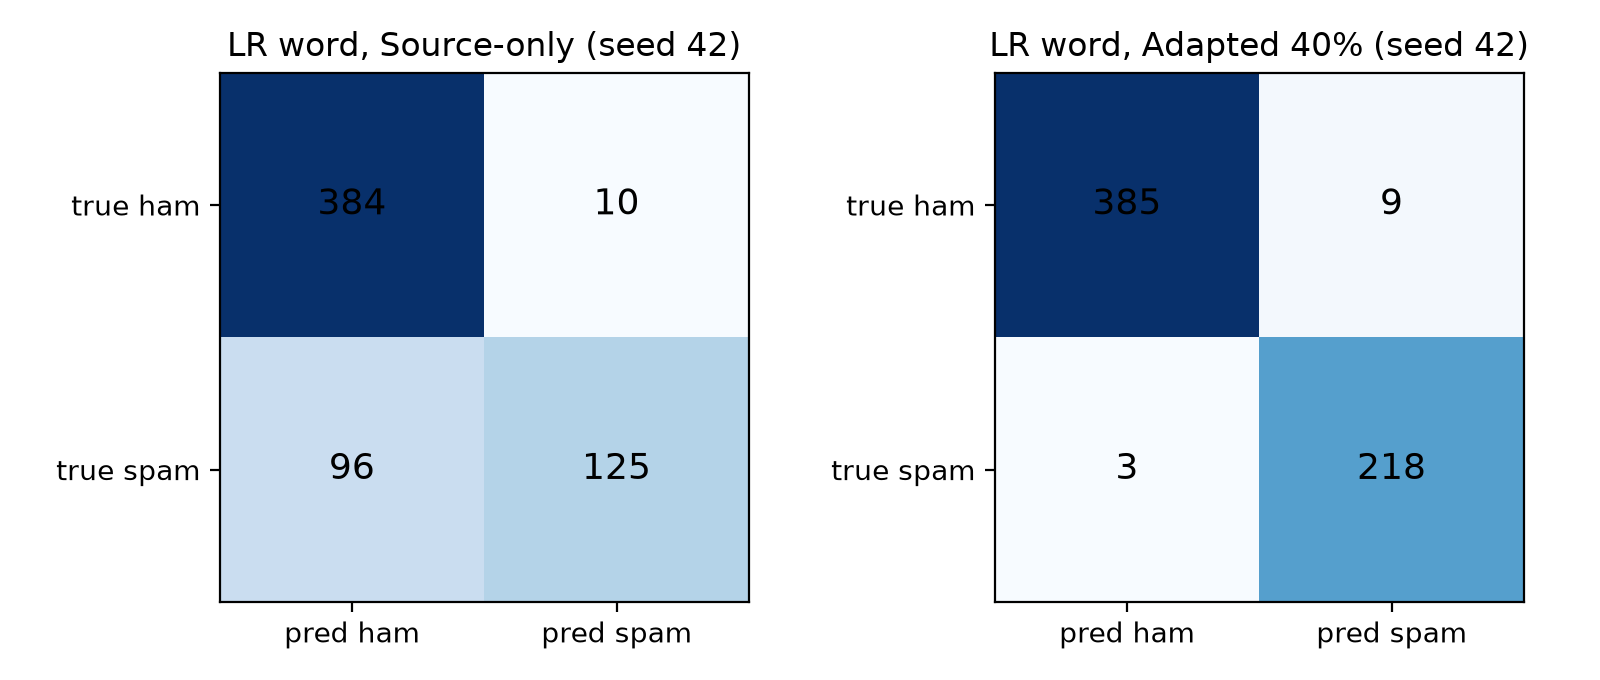
\includegraphics[width=0.92\columnwidth]{figures/fig7_confusion_matrices.png}
\caption{Logistic Regression (word TF-IDF, seed 42) on the 615-message final target test set, before and after adding 40\% of the pool.}
\label{fig:cm}
\end{figure}

\subsection{Is the Gain Caused by Near-Duplicates?}
Indian promotional SMS are sent from templates, so a random 70/30 split can put a near-copy of a test message into the adaptation pool. We grouped Dataset B into near-duplicate groups with MinHash~\cite{broder1997} (estimated Jaccard similarity $\ge 0.6$ on word 3-shingles after replacing links and digits), giving 1,811 groups for 2,050 messages. Under the random split, 86--104 of the 615 test messages (59--69 of the 221 spam) had a near-copy in the pool. We then repeated adaptation with a group-aware split that keeps each group on one side. Table~\ref{tab:group} shows that the gains shrink only slightly: with 10\% of the pool, Logistic Regression reaches 0.952 instead of 0.964. The adaptation effect is therefore not explained by memorised templates.

\begin{table}[t]
\centering
\caption{Target F1 with a random and a group-aware split of Dataset B (word TF-IDF, mean $\pm$ SD)}
\label{tab:group}
\begin{tabular}{llcc}
\toprule
Model & Added & Random split & Group-aware \\
\midrule
\multirow{2}{*}{Logistic Reg.} & 0\% & 0.681 $\pm$ 0.025 & 0.652 $\pm$ 0.062 \\
 & 10\% & 0.964 $\pm$ 0.004 & 0.952 $\pm$ 0.008 \\
 & 40\% & 0.975 $\pm$ 0.005 & 0.969 $\pm$ 0.011 \\
\midrule
\multirow{2}{*}{Naive Bayes} & 0\% & 0.582 $\pm$ 0.018 & 0.551 $\pm$ 0.017 \\
 & 10\% & 0.950 $\pm$ 0.006 & 0.937 $\pm$ 0.015 \\
 & 40\% & 0.978 $\pm$ 0.009 & 0.960 $\pm$ 0.015 \\
\bottomrule
\end{tabular}
\end{table}

\subsection{RQ3: Word versus Character Features}
Neither representation won for both classifiers (Table~\ref{tab:feat}). Character n-grams improved source-only target F1 for Naive Bayes (0.582 $\to$ 0.704), consistent with their tolerance to spelling and formatting variation, but lowered it slightly for Logistic Regression (0.681 $\to$ 0.658), whose target recall fell. After adaptation the two representations are within 0.01 of each other for Logistic Regression.

\begin{table}[t]
\centering
\caption{Source-only models: word versus character TF-IDF (mean $\pm$ SD)}
\label{tab:feat}
\begin{tabular}{llccc}
\toprule
Model & Feature & Source F1 & Target F1 & Target rec. \\
\midrule
\multirow{2}{*}{Naive Bayes} & word & 0.927 & 0.582 $\pm$ 0.018 & 0.430 \\
 & char & 0.941 & 0.704 $\pm$ 0.017 & 0.581 \\
\multirow{2}{*}{Logistic Reg.} & word & 0.928 & 0.681 $\pm$ 0.025 & 0.535 \\
 & char & 0.942 & 0.658 $\pm$ 0.027 & 0.502 \\
\bottomrule
\end{tabular}
\end{table}

\subsection{RQ5: What Differs Between the Domains}
On average, 20.7\% of the words in an Indian message never occur in the UCI training split, against 7.8\% for held-out UCI messages. Indian messages are longer (median 81 against 59 characters), and Indian spam is longer still (median 153). 87.0\% of Indian spam contains a URL and 24.3\% a currency marker such as ``Rs'' or ``INR'', whereas only 1.6\% of UCI test messages contain a URL. The UCI-trained models therefore meet spam vocabulary they never saw (``cashback'', ``NeuCoins'', ``recharge'', brand and app names) and spam formats they never learned. We read all 118 errors of Logistic Regression (word TF-IDF, seed 42) one by one. Of the 106 source-only errors, 61 are Indian brand or telecom promotions whose vocabulary the UCI model never saw, 14 are operator service notices (data alerts, pack expiry, missed-call alerts), 6 are fraudulent ``wallet credit'' messages with digit-for-letter spelling (``t0'', ``n0w''), 3 are loan or debt messages, 2 are code-mixed Hinglish promotions and 8 are very short chat messages (false alarms). Nine are questionable labels: safety advice, receipts and feedback requests labelled spam in Dataset B. After adaptation only 12 errors remain: 8 very short chat messages such as ``join from'' or ``now*'', two disguised-spelling frauds, one market commentary and one questionable label. The remaining errors therefore come from messages that carry almost no content or from labels that are themselves doubtful.

\section{Limitations}
The study uses two datasets, so it cannot claim robustness across domains in general. Dataset B is a public, crowd-sourced collection without a documented labelling procedure, and its genuine messages are mostly short chat; it does not represent all Indian SMS traffic. One property of Dataset B makes adaptation easier: none of its ham messages contains a URL, while 87\% of its spam does, so an adapted model can partly rely on that cue. Three seeds give a limited estimate of variability, and the error categories await manual verification. Finally, ``spam'' here includes legitimate brand promotions; detecting fraud specifically would need different labels.

\section{Conclusion and Future Work}
A conventional SMS spam classifier trained on UK messages loses 0.23--0.36 F1 on Indian messages, mainly by missing spam. Logistic Regression with word TF-IDF transferred best, and Naive Bayes transferred only when its smoothing was chosen properly. Adding as few as 143 labelled Indian messages to the training data restored target F1 above 0.95 for both models without harming source performance, consistently across seeds and significantly by McNemar's test, and the gain survived a split that keeps near-duplicates apart. Character n-grams helped Naive Bayes but not Logistic Regression. The practical message is that a small, carefully labelled local sample is worth more than a choice between conventional models. Future work includes a second target dataset, more seeds, a learning curve below 10\%, label verification by a second annotator, and transformer models under the same protocol.

\section*{Data and Code Availability}
The notebook, cleaned datasets, result tables, saved models and the demonstration application are in the project repository (\url{https://github.com/priyamthakur275/ScamGuard-AI}, directory \texttt{research/cross\_domain}).

\balance
\begin{thebibliography}{99}
\bibitem{almeida2011} T.~A. Almeida, J.~M. G\'omez Hidalgo, and A.~Yamakami, ``Contributions to the study of SMS spam filtering: New collection and results,'' in \textit{Proc. 11th ACM Symp. Document Engineering (DocEng)}, 2011, pp.~259--262, doi: 10.1145/2034691.2034742.
\bibitem{almeida2013} T.~A. Almeida, J.~M. G\'omez Hidalgo, and T.~P. Silva, ``Towards SMS spam filtering: Results under a new dataset,'' \textit{Int. J. Information Security Science}, vol.~2, no.~1, pp.~1--18, 2013.
\bibitem{roy2020} P.~K. Roy, J.~P. Singh, and S.~Banerjee, ``Deep learning to filter SMS spam,'' \textit{Future Generation Computer Systems}, vol.~102, pp.~524--533, 2020, doi: 10.1016/j.future.2019.09.001.
\bibitem{indiasms} JuniorAlive, ``India Spam SMS Classification,'' GitHub repository, 2024. [Online]. Available: https://github.com/junioralive/india-spam-sms-classification
\bibitem{bendavid2010} S.~Ben-David, J.~Blitzer, K.~Crammer, A.~Kulesza, F.~Pereira, and J.~W. Vaughan, ``A theory of learning from different domains,'' \textit{Machine Learning}, vol.~79, pp.~151--175, 2010, doi: 10.1007/s10994-009-5152-4.
\bibitem{pan2010} S.~J. Pan and Q.~Yang, ``A survey on transfer learning,'' \textit{IEEE Trans. Knowledge and Data Engineering}, vol.~22, no.~10, pp.~1345--1359, 2010, doi: 10.1109/TKDE.2009.191.
\bibitem{daume2007} H.~Daum\'e~III, ``Frustratingly easy domain adaptation,'' in \textit{Proc. 45th Annu. Meeting Assoc. Computational Linguistics (ACL)}, 2007, pp.~256--263.
\bibitem{lee2022} K.~Lee, D.~Ippolito, A.~Nystrom, C.~Zhang, D.~Eck, C.~Callison-Burch, and N.~Carlini, ``Deduplicating training data makes language models better,'' in \textit{Proc. 60th Annu. Meeting ACL}, 2022, pp.~8424--8445, doi: 10.18653/v1/2022.acl-long.577.
\bibitem{kapoor2023} S.~Kapoor and A.~Narayanan, ``Leakage and the reproducibility crisis in machine-learning-based science,'' \textit{Patterns}, vol.~4, no.~9, 2023, doi: 10.1016/j.patter.2023.100804.
\bibitem{salton1988} G.~Salton and C.~Buckley, ``Term-weighting approaches in automatic text retrieval,'' \textit{Information Processing \& Management}, vol.~24, no.~5, pp.~513--523, 1988, doi: 10.1016/0306-4573(88)90021-0.
\bibitem{pedregosa2011} F.~Pedregosa \textit{et al.}, ``Scikit-learn: Machine learning in Python,'' \textit{J. Machine Learning Research}, vol.~12, pp.~2825--2830, 2011.
\bibitem{mcnemar1947} Q.~McNemar, ``Note on the sampling error of the difference between correlated proportions or percentages,'' \textit{Psychometrika}, vol.~12, no.~2, pp.~153--157, 1947, doi: 10.1007/BF02295996.
\bibitem{dietterich1998} T.~G. Dietterich, ``Approximate statistical tests for comparing supervised classification learning algorithms,'' \textit{Neural Computation}, vol.~10, no.~7, pp.~1895--1923, 1998, doi: 10.1162/089976698300017197.
\bibitem{broder1997} A.~Z. Broder, ``On the resemblance and containment of documents,'' in \textit{Proc. Compression and Complexity of SEQUENCES}, 1997, pp.~21--29, doi: 10.1109/SEQUEN.1997.666900.
\end{thebibliography}
\end{document}
